\subsection{Behavioral Patterns}

\frame{\tableofcontents[currentsection, currentsubsection]}


\begin{frame}[t]{Template Method}
	\stress{\badc{Questionable:}}
	\inputminted{python}{code/patterns/behavioral/template_method_bad.py}
	\only<2->{
		\begin{itemize}
			\item What if multiple methods depend on the model? \srem{$\lra$ Need to keep track of more \texttt{if}s everywhere}
			\item What if we want to add or remove a model? \srem{$\lra$ Need to make changes in many places $\lra$ \sout{Open/Closed Principle}}, \enquote{divergent change}
			\item Depend on all implementations $\lra$ \srem{\sout{Dependency Inversion Principle}}
		\end{itemize}
	}
\end{frame}


\begin{frame}{Template Method}
	\begin{itemize}[<+->]
		\item \hhl{Use case:} Several different algorithms that only contain minor differences in few places
		\item \hhl{Suggestion:} Put shared code in superclass, have subclasses implement or override specific methods
		
		\begin{center}
		\begin{tikzpicture}[scale=0.7, transform shape]
		\umlclass[x=0,y=3, type=abstract]{MLModel}{ 
		}{ 
			+ preprocess()\\ 
			\emph{+ train()}\\ 
			+ validate()
		} 
		
		\umlclass[x=-2,y=0]{BDT}{}{+ train()}
		\umlinherit{BDT}{MLModel}
		
		\umlclass[x=2,y=0]{RandomForest}{}{+ train()}
		\umlinherit{RandomForest}{MLModel}
		\end{tikzpicture}
		\end{center}
		\item \hhl{Advantages:} Simple and clean with little overhead
		\item \hhl{Warnings:} 
		\begin{itemize}
			\item If there are many differences between original classes, we need (to override) many methods $\lra$ increasingly hard to read and mantain
			\item If there are multiple \enquote{options} for every method and we want to realize them, the number of subclasses grows exponentially $\lra$ \emph{Strategy pattern}
			\item If overriding default methods, the Liskov Substitution Principle can be easily violated
		\end{itemize}
	\end{itemize}
	%
	
\end{frame}

\begin{frame}{Template Method}
	\stress{\goodc{Better:}}
	\inputminted{python}{code/patterns/behavioral/template_method.py}
\end{frame}

\begin{frame}{Strategy}
	\begin{itemize}[<+->]
		%
		\item 
		\hhl{Usage:} Your problem consists of several steps. Each step can be solved with different algorithms (strategies)
		%
		\item 
		\hhl{Suggestion:} Create abstract class for each step and concrete subclasses with specific algorithms; original class holds instances of algorithms
		
		\begin{center}
			\begin{tikzpicture}[scale=0.7, transform shape]
			\umlclass[x=0,y=3]{MyAnalysis}{ 
				+ ml\_model: MLModel\\
				+ fitter: Fitter
			}{ 
				%\dots\\
				+ train()\\
				+ fit()\\
				%\dots
			} 
			
			\umlclass[y=3, x=4, type=abstract]{MLModel}{}{\emph{+ train()}}
			\umlaggreg{MyAnalysis}{MLModel}
			
			\umlclass[x=2,y=0]{BDT}{}{+ train()}
			\umlinherit{BDT}{MLModel}
			
			\umlclass[x=6,y=0]{RandomForest}{}{+ train()}
			\umlinherit{RandomForest}{MLModel}
			
			\umlclass[y=3, x=-4, type=abstract]{Fitter}{}{\emph{+ fit()}}
			\umlaggreg{MyAnalysis}{Fitter}
			
			\umlclass[x=-5,y=0]{KernelDensityFit}{}{+ fit()}
			\umlinherit{KernelDensityFit}{Fitter}
			
			\umlclass[x=-2,y=0]{CrystalBallFit}{}{+ fit()}
			\umlinherit{CrystalBallFit}{Fitter}
			\end{tikzpicture}
		\end{center}
	\end{itemize}
\end{frame}

\begin{frame}{Strategy}
	\inputminted{python}{code/patterns/behavioral/strategy.py}
\end{frame}

\begin{frame}{Strategy}
	\begin{itemize}
		\item<1-> \hhl{Note}: The main class holds instances of algorithm classes; the algorithm classes use the the \hl{template method} pattern
		\item<2-> \hhl{Advantages}:
		\begin{itemize}[]
			\item \hl{Open/Closed} principle: Easily add new strategies
			\item \hl{Dependencies inverted} (\texttt{MyAnalysis} does not depend on the individual implementations)
			\item \hl{Small number of subclasses}
			\item \hl{Separated implementation} of algorithms from higher level code
			\item For compiled languages: Change algorithms at \hl{runtime}
		\end{itemize}
		\item<3-> \hhl{Warnings}: 
			\begin{itemize}
				\item Might be overkill for very simple problems
				\item For maximum performance, avoid virtual calls
			\end{itemize}
		\item<4-> \hhl{Alternatives}:
		\begin{itemize}
			\item If your language supports it: Use functions instead of objects \srem{(e.g. provide several \texttt{fit()} functions and pass them to the class)}
			\item Use template pattern if there is only one strategy that can be replaced
		\end{itemize}
	\end{itemize}
\end{frame}

\begin{frame}[t]{Command}
	\begin{quote}
	The command pattern turns a \hhl{method call} into a \hhl{standalone object}.
	\end{quote}
	
	\medskip
	Rather than directly calling a method, the interface creates a \texttt{Command} object \srem{(describing what we want to execute)} and passing it on to a \texttt{Receiver} that executes it
	
	\only<2->{
		\bigskip
		Use cases:
		\begin{itemize}
			\item<2-> \hhl{Decouple} user interfaces from the backend \srem{(by using \texttt{Command} objects as means of communication)}
			\item<3-> Build up a command \hhl{history} with \hhl{undo} functionality
			\item<4-> \hhl{Remote execution} of commands
			\item<5-> \hhl{Queue} or \hhl{schedule} operations
			%\end{itemize}
		\end{itemize}
	}
	\only<6->{
		\bigskip
		HEP specific use case example (Belle II software framework):
		\begin{itemize}
			\item<7-> Build up analysis by adding modules \srem{(\texttt{Command} objects)} to a path \srem{(list of modules)}, each implementing a \texttt{event()} method to process one event
			\item<8-> After all modules are added, process the path: Loop over all events, calling the \texttt{event()} method of all modules in order
		\end{itemize}
	}
\end{frame}

\begin{frame}{Command}
	Slightly simplified Belle II steering file:
	
	\inputminted[fontsize=\small]{python}{code/patterns/behavioral/belle2_steering_file.py}
\end{frame}

\begin{frame}{Command}
	Upon processing path:
	%
	\begin{center}
	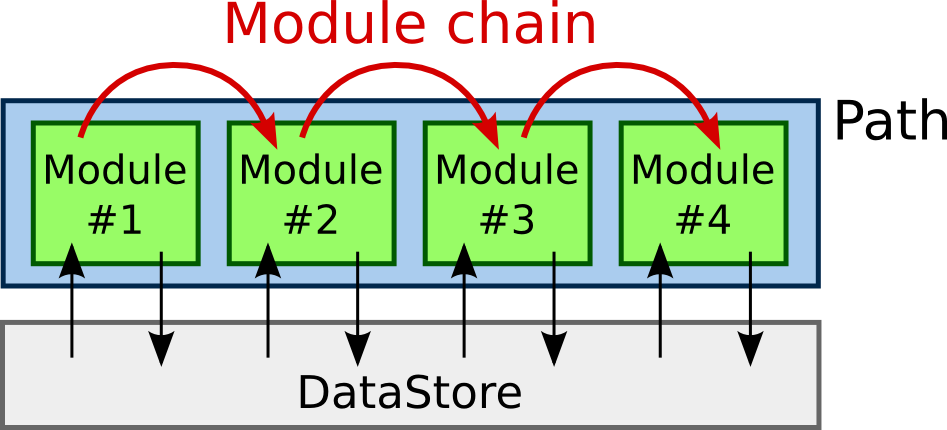
\includegraphics[height=3.5cm]{figures/patterns/behavioral/ModulePath.png}
	\end{center}
	
	\bigskip
	\begin{itemize}[<+->]
		\item Strictly \hhl{declarative} approach \srem{(no for loops or implementation details)}
		\item Modules can be implemented in \proglang{python} or \proglang{C++}
		\item \hhl{\enquote{Building block}} approach makes steering files extremely easy to write and understand \srem{(even browser based graphical interface for highschoolers: try it at \url{masterclass.ijs.si})}
	\end{itemize}
\end{frame}

%\begin{frame}{Iterator}
%	
%\end{frame}

\begin{frame}{Visitor}
	\begin{itemize}
		\item 
		\hhl{Concrete example}: Serialize a collection of instances of different classes \srem{(e.g. provide JSON export for a list  of different data objects)}
		\item
		\hhl{Possible implementation}: Provide a \texttt{to\_json()} method to all classes
		\item 
		\hhl{Potential issue}: 
		Might soon want to add export for export possibilities: \srem{(\texttt{XML}, \texttt{CSV}, \texttt{YAML}, etc.)}
		\Lrapar{more and more unrelated methods need to be added to the data class}
		\Lrapar{\hl{\enquote{polluted} interface} \srem{(methods are irrelevant for core functionality)}; people might be wary of \hl{frequent changes} to a well working class}
		\item 
		\hhl{Solution}: 
		Separate algorithms from the objects they operate on
		\medskip
		\begin{center}
			\begin{tikzpicture}[scale=0.7, transform shape]
			\umlclass[x=-2,y=3, type=abstract]{Visitor}{ 
				
			}{ 
				+ \emph{visit\_element\_a()}\\
				+ \emph{visit\_element\_b()}
			} 
			
			\umlemptyclass[x=-2,y=0]{JSONExport}
			\umlinherit{JSONExport}{Visitor}
			
			\umlclass[y=3,x=5, type=abstract]{Element}{ 
			}{ 
				+ \emph{accept(visitor)}\\ 
			} 
			
			\umlclass[y=0,x=3.5]{ElementA}{}{+ accept(visitor)}
			\umlVHVinherit{ElementA}{Element}
			\umluniassoc[geometry=-|-, anchor1=-160, anchor2=-8]{ElementA}{Visitor}
			
			
			\umlclass[y=0,x=6.5]{ElementB}{}{+ accept(visitor)}
			\umlVHVinherit{ElementB}{Element}
			\umluniassoc[anchor1=-160, anchor2=-22]{ElementB}{Visitor}
			\end{tikzpicture}
		\end{center}
	\end{itemize}
\end{frame}

\begin{frame}{Visitor}
	\hhl{Use case} \srem{(more formally)}:
	\begin{itemize}
		\item<2-> Given a heterogeneous family of \texttt{Element} classes
		\item<2-> Do not expect significant changes to \texttt{Element} classes 
		\item<3-> Various unrelated operations need to be performed on a collection of \texttt{Element} objects
		\item<3-> We expect frequent additions and changes for the operations
		\item<3-> Do not want to frequently change \texttt{Element} classes because of that 
		\end{itemize}
	
	\bigskip
	\hhl{Advantages of visitor pattern}:
	\begin{itemize}
		\item<4-> Single responsibility principle: All the operation functionality is in one place
		\item<4-> Open/Closed principle: Easy to add new operations
	\end{itemize}
	
	\bigskip
	\hhl{Disadvantages of the visitor pattern}:
	\begin{itemize}[<+->]
		\item<5-> No access to private information of \texttt{Element} classes
		\item<6-> Changes to \texttt{Element} classes can require changes to all visitors
	\end{itemize}
\end{frame}